\documentclass[a4paper,11pt,openright]{report}
\setlength{\parindent}{0pt} % set noindent for entire file

\usepackage[utf8]{inputenc}
\usepackage[a4paper,top=25mm,bottom=25mm,left=15mm,right=20mm]{geometry}
\usepackage{xcolor,graphicx}
\usepackage{amsmath}
\usepackage{setspace}
\usepackage{sectsty}
\usepackage{etoolbox}
\usepackage{enumitem}
\usepackage{listings}
\usepackage{textcmds}
\usepackage{times}

\graphicspath{ {/home/saran/Analytics/Jun_30/} }

\lstdefinestyle{mystyle}{
	backgroundcolor=\color{white},
	basicstyle=\ttfamily\footnotesize,
	breakatwhitespace=false,
	breaklines=true,
	captionpos=b,
	keepspaces=true,
	showspaces=false,
	showstringspaces=false,
	showtabs=false,
	tabsize=4
}

\lstset{style=mystyle}

\begin{document}
\singlespacing
\pagestyle{plain}

\begin{small}
\begin{center}
\textbf{Assignment: GridFS} \\
Date: 21/10/2020 \hspace{2mm} Name: D.Saravanan
\end{center}
\end{small}

\vspace{10px}

\begin{footnotesize}
1. Using GridFS insert some files in your database. Display the information of your files
using fs.files and fs.chunks.
\end{footnotesize}

{\footnotesize Import file zips.json}
%figure_1
\begin{figure}[ht!]
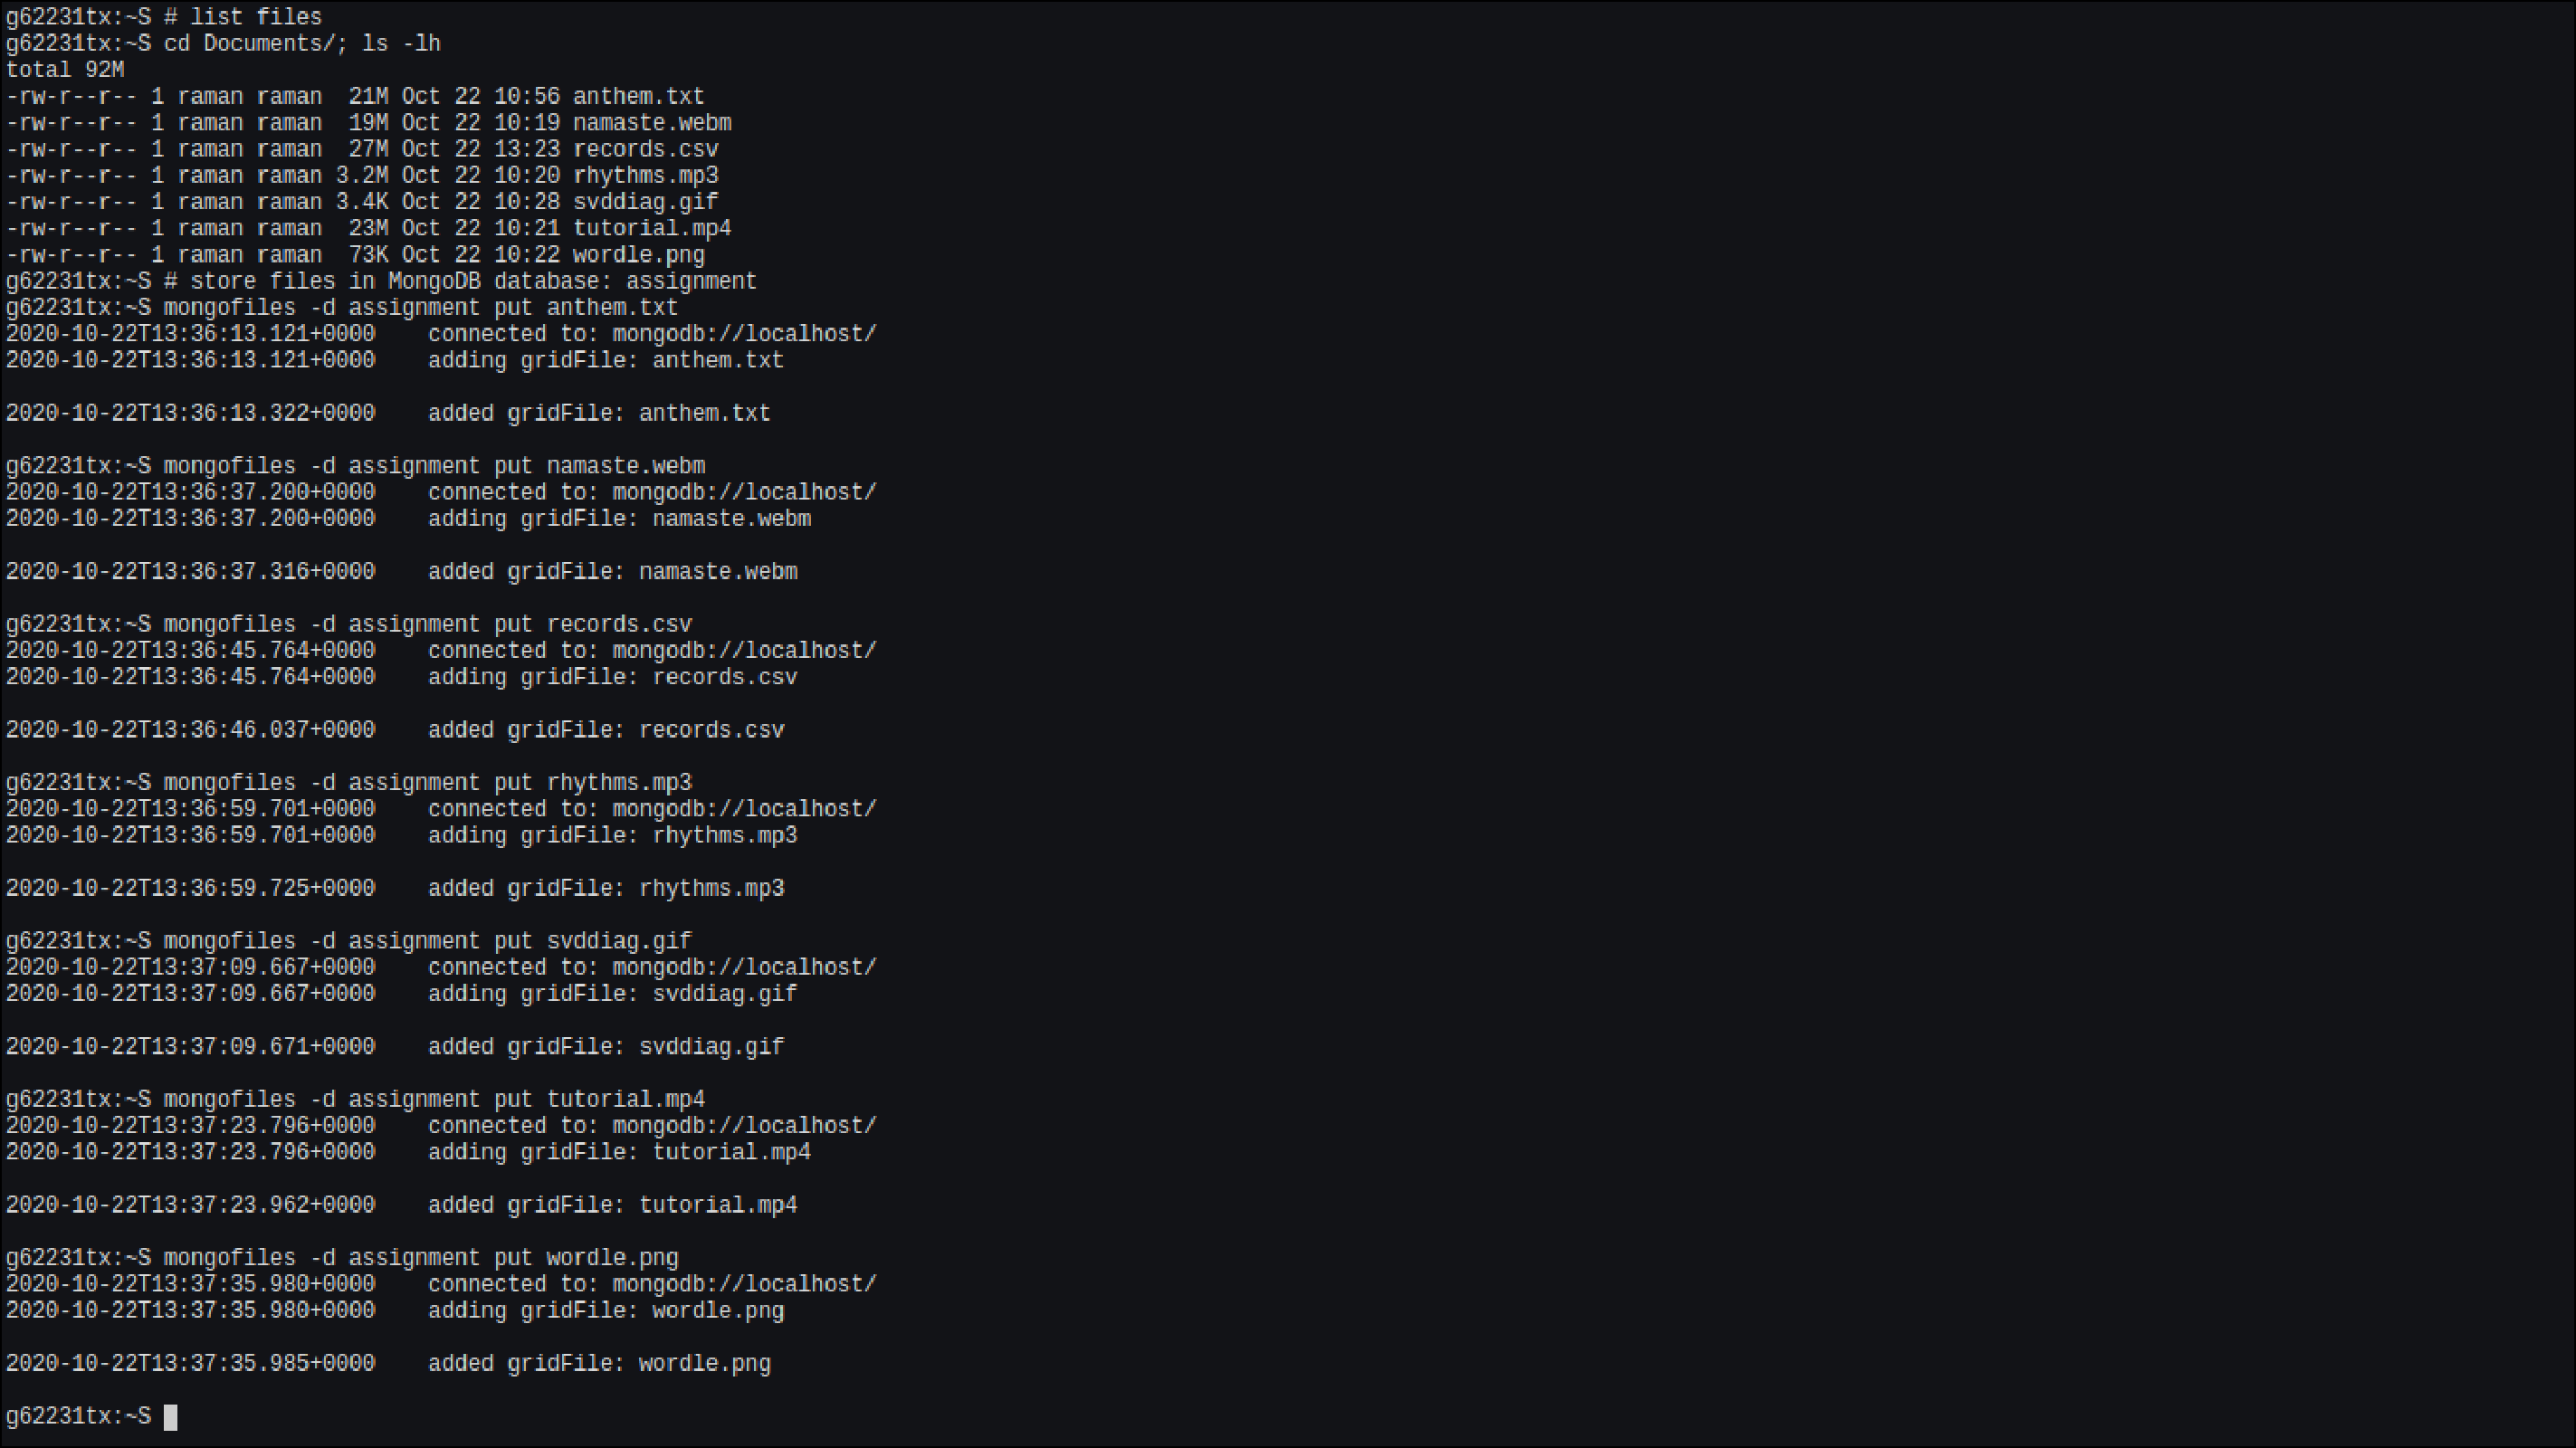
\includegraphics[width=20cm,height=10cm,keepaspectratio]{image1.pdf}
\centering
\end{figure}

%{\footnotesize ZipCode collection}
%%figure_2
%\begin{figure}[ht!]
%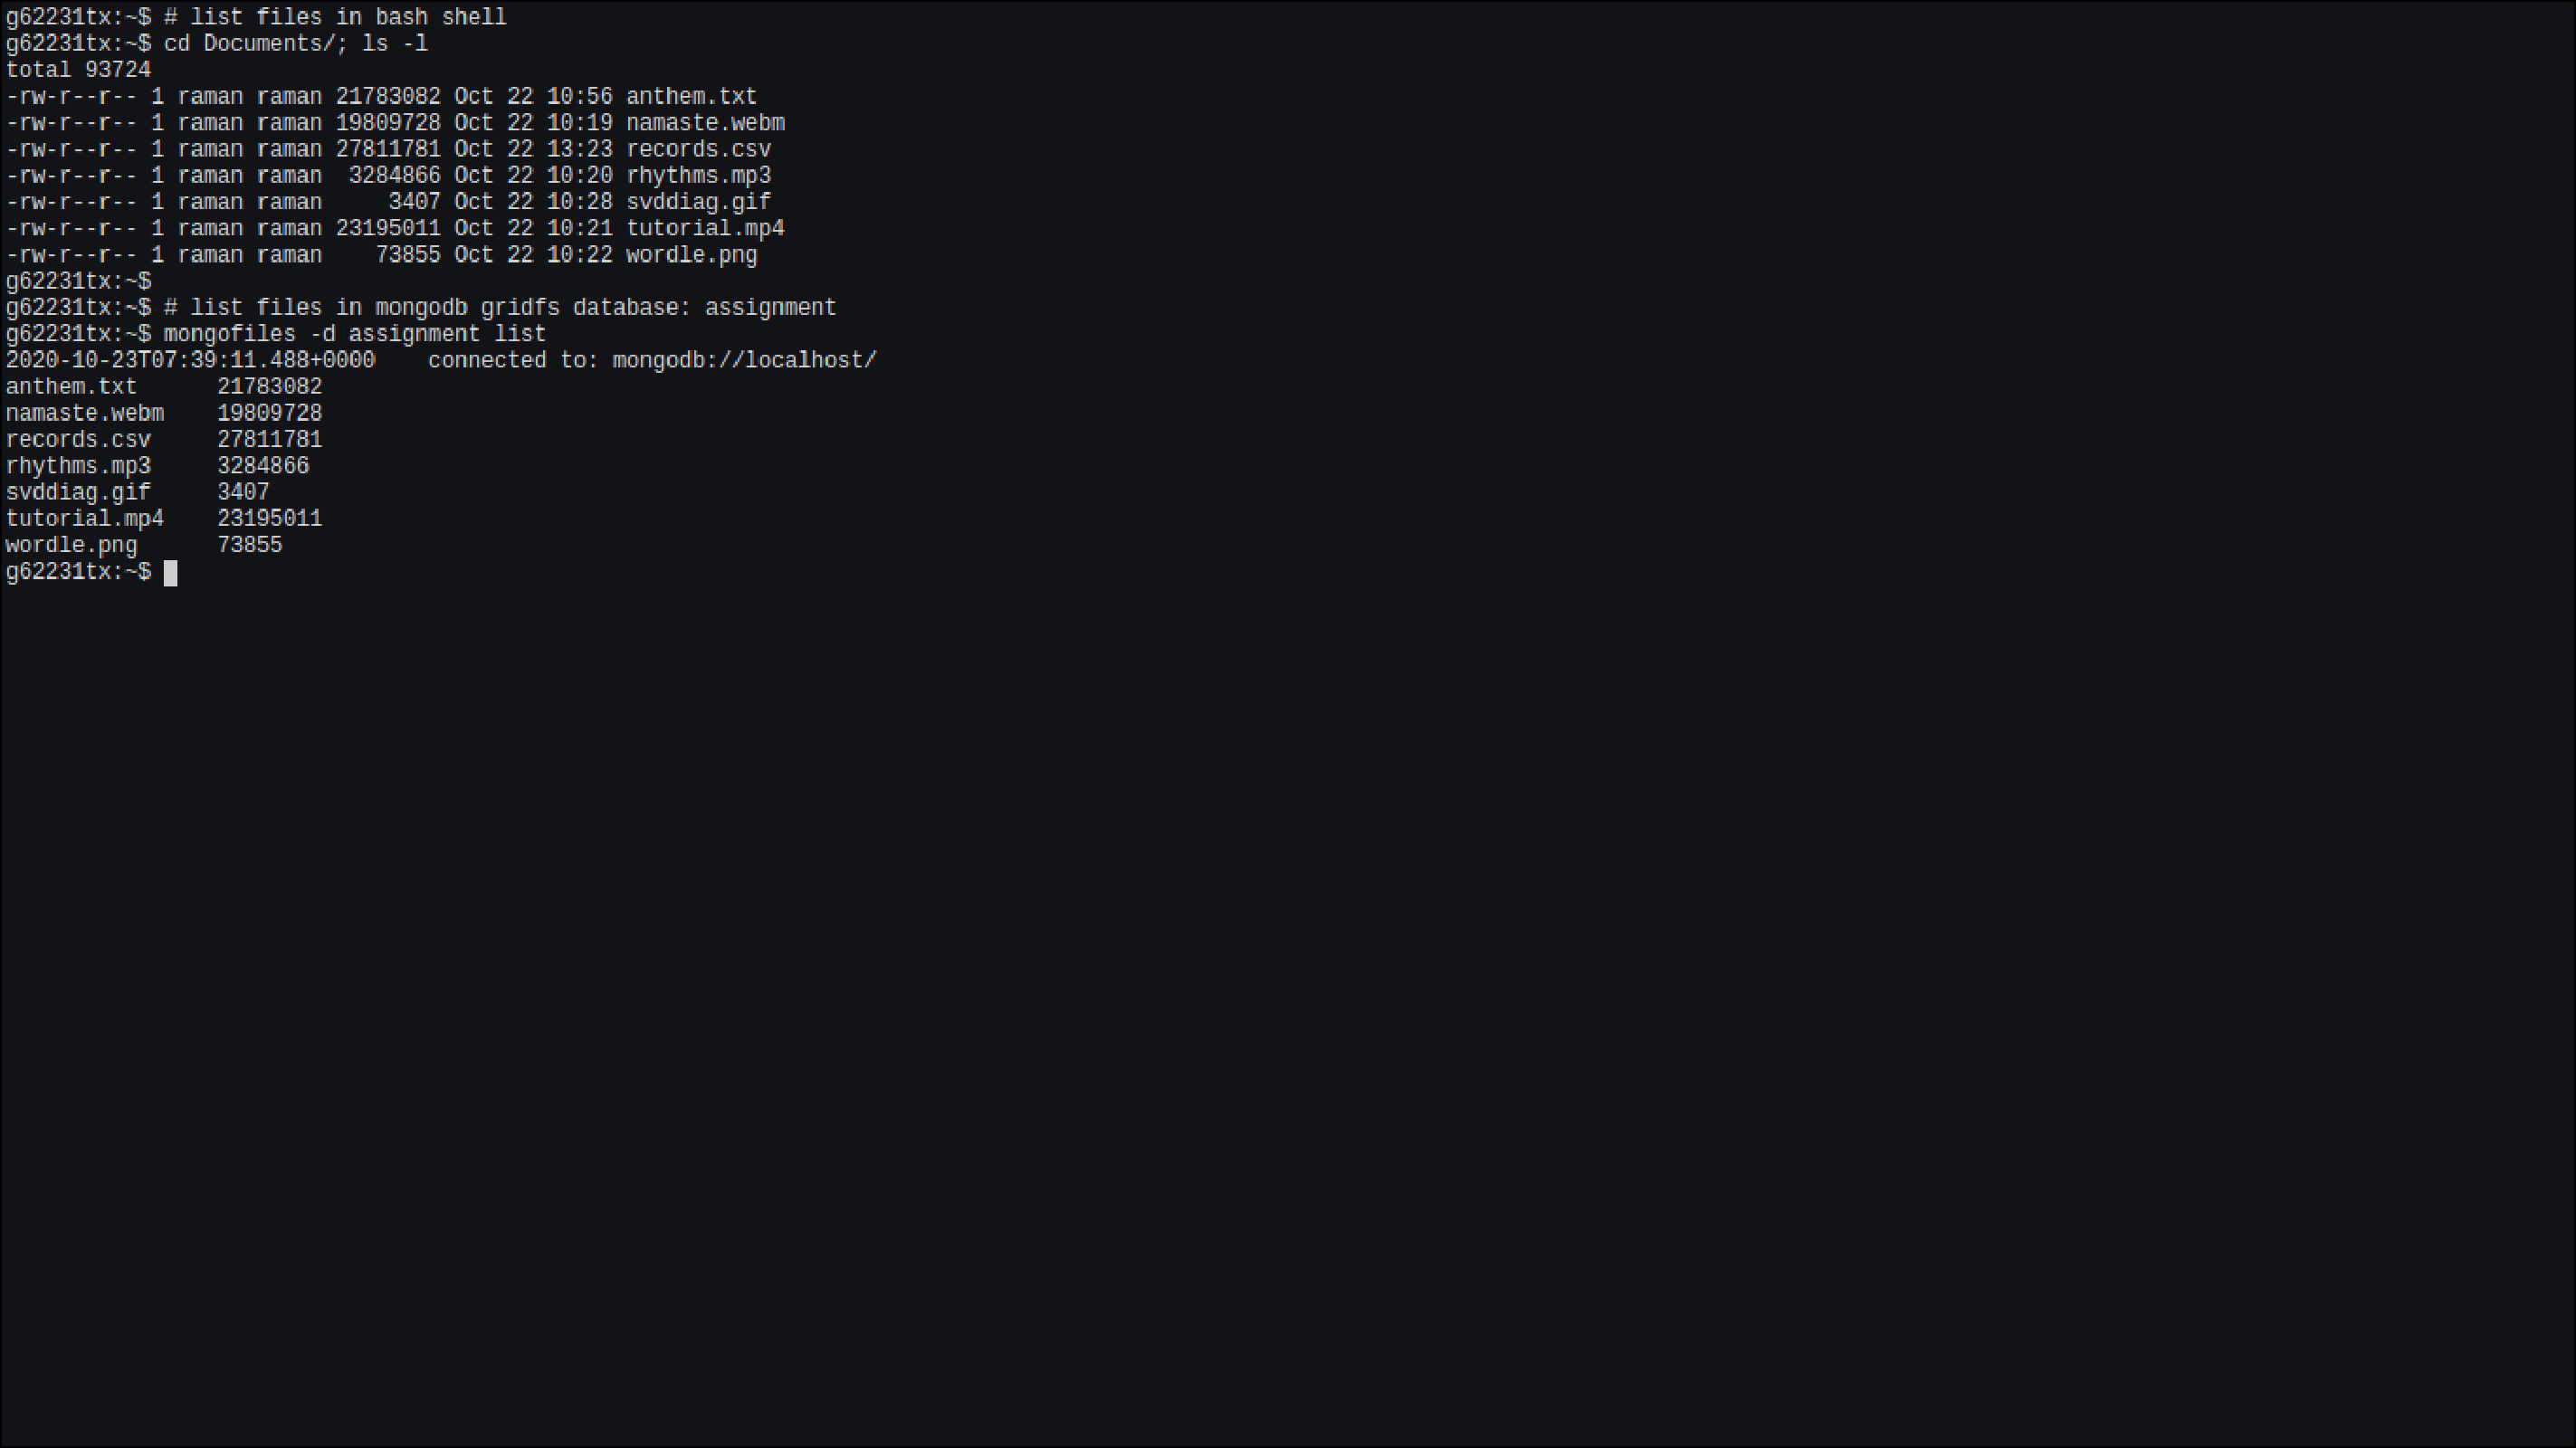
\includegraphics[width=20cm,height=10cm,keepaspectratio]{image2.pdf}
%\centering
%\end{figure}
%
%\pagebreak
%
%{\footnotesize $\$$project}
%%figure_3
%\begin{figure}[ht!]
%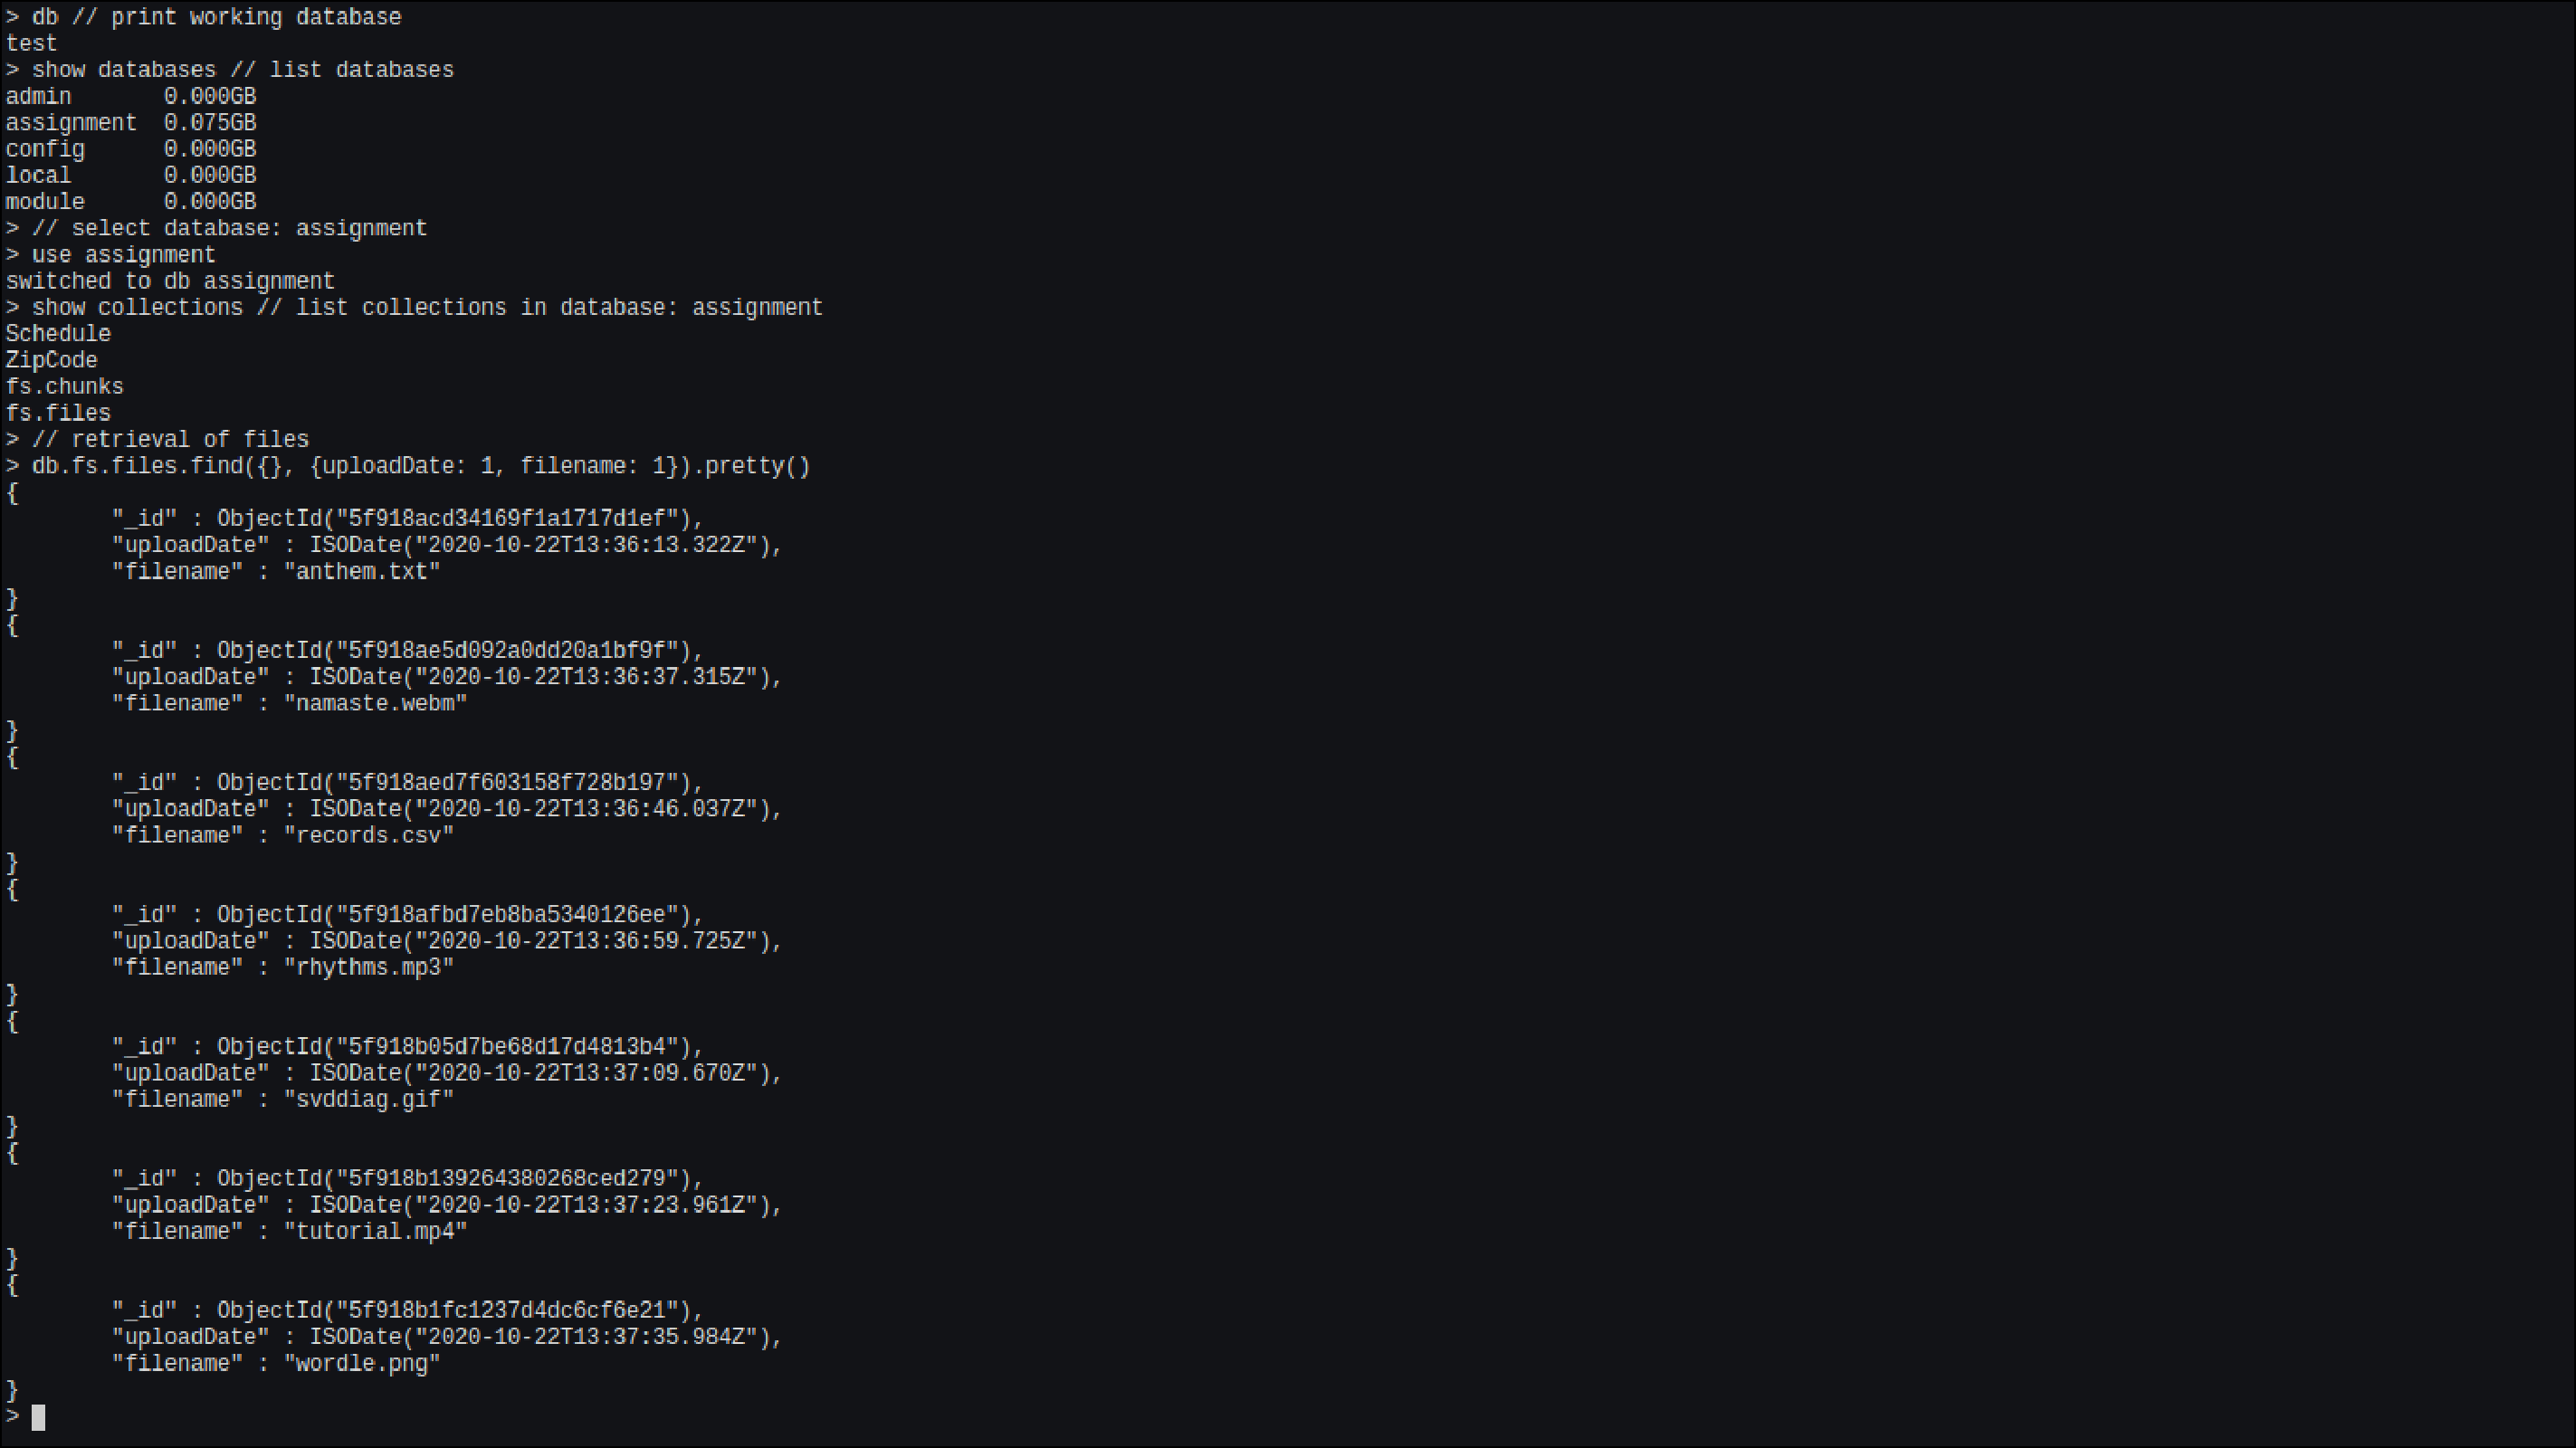
\includegraphics[width=20cm,height=10cm,keepaspectratio]{image3.pdf}
%\centering
%\end{figure}
%
%\vspace{20px}
%
%{\footnotesize $\$$match}
%%figure_4
%\begin{figure}[ht!]
%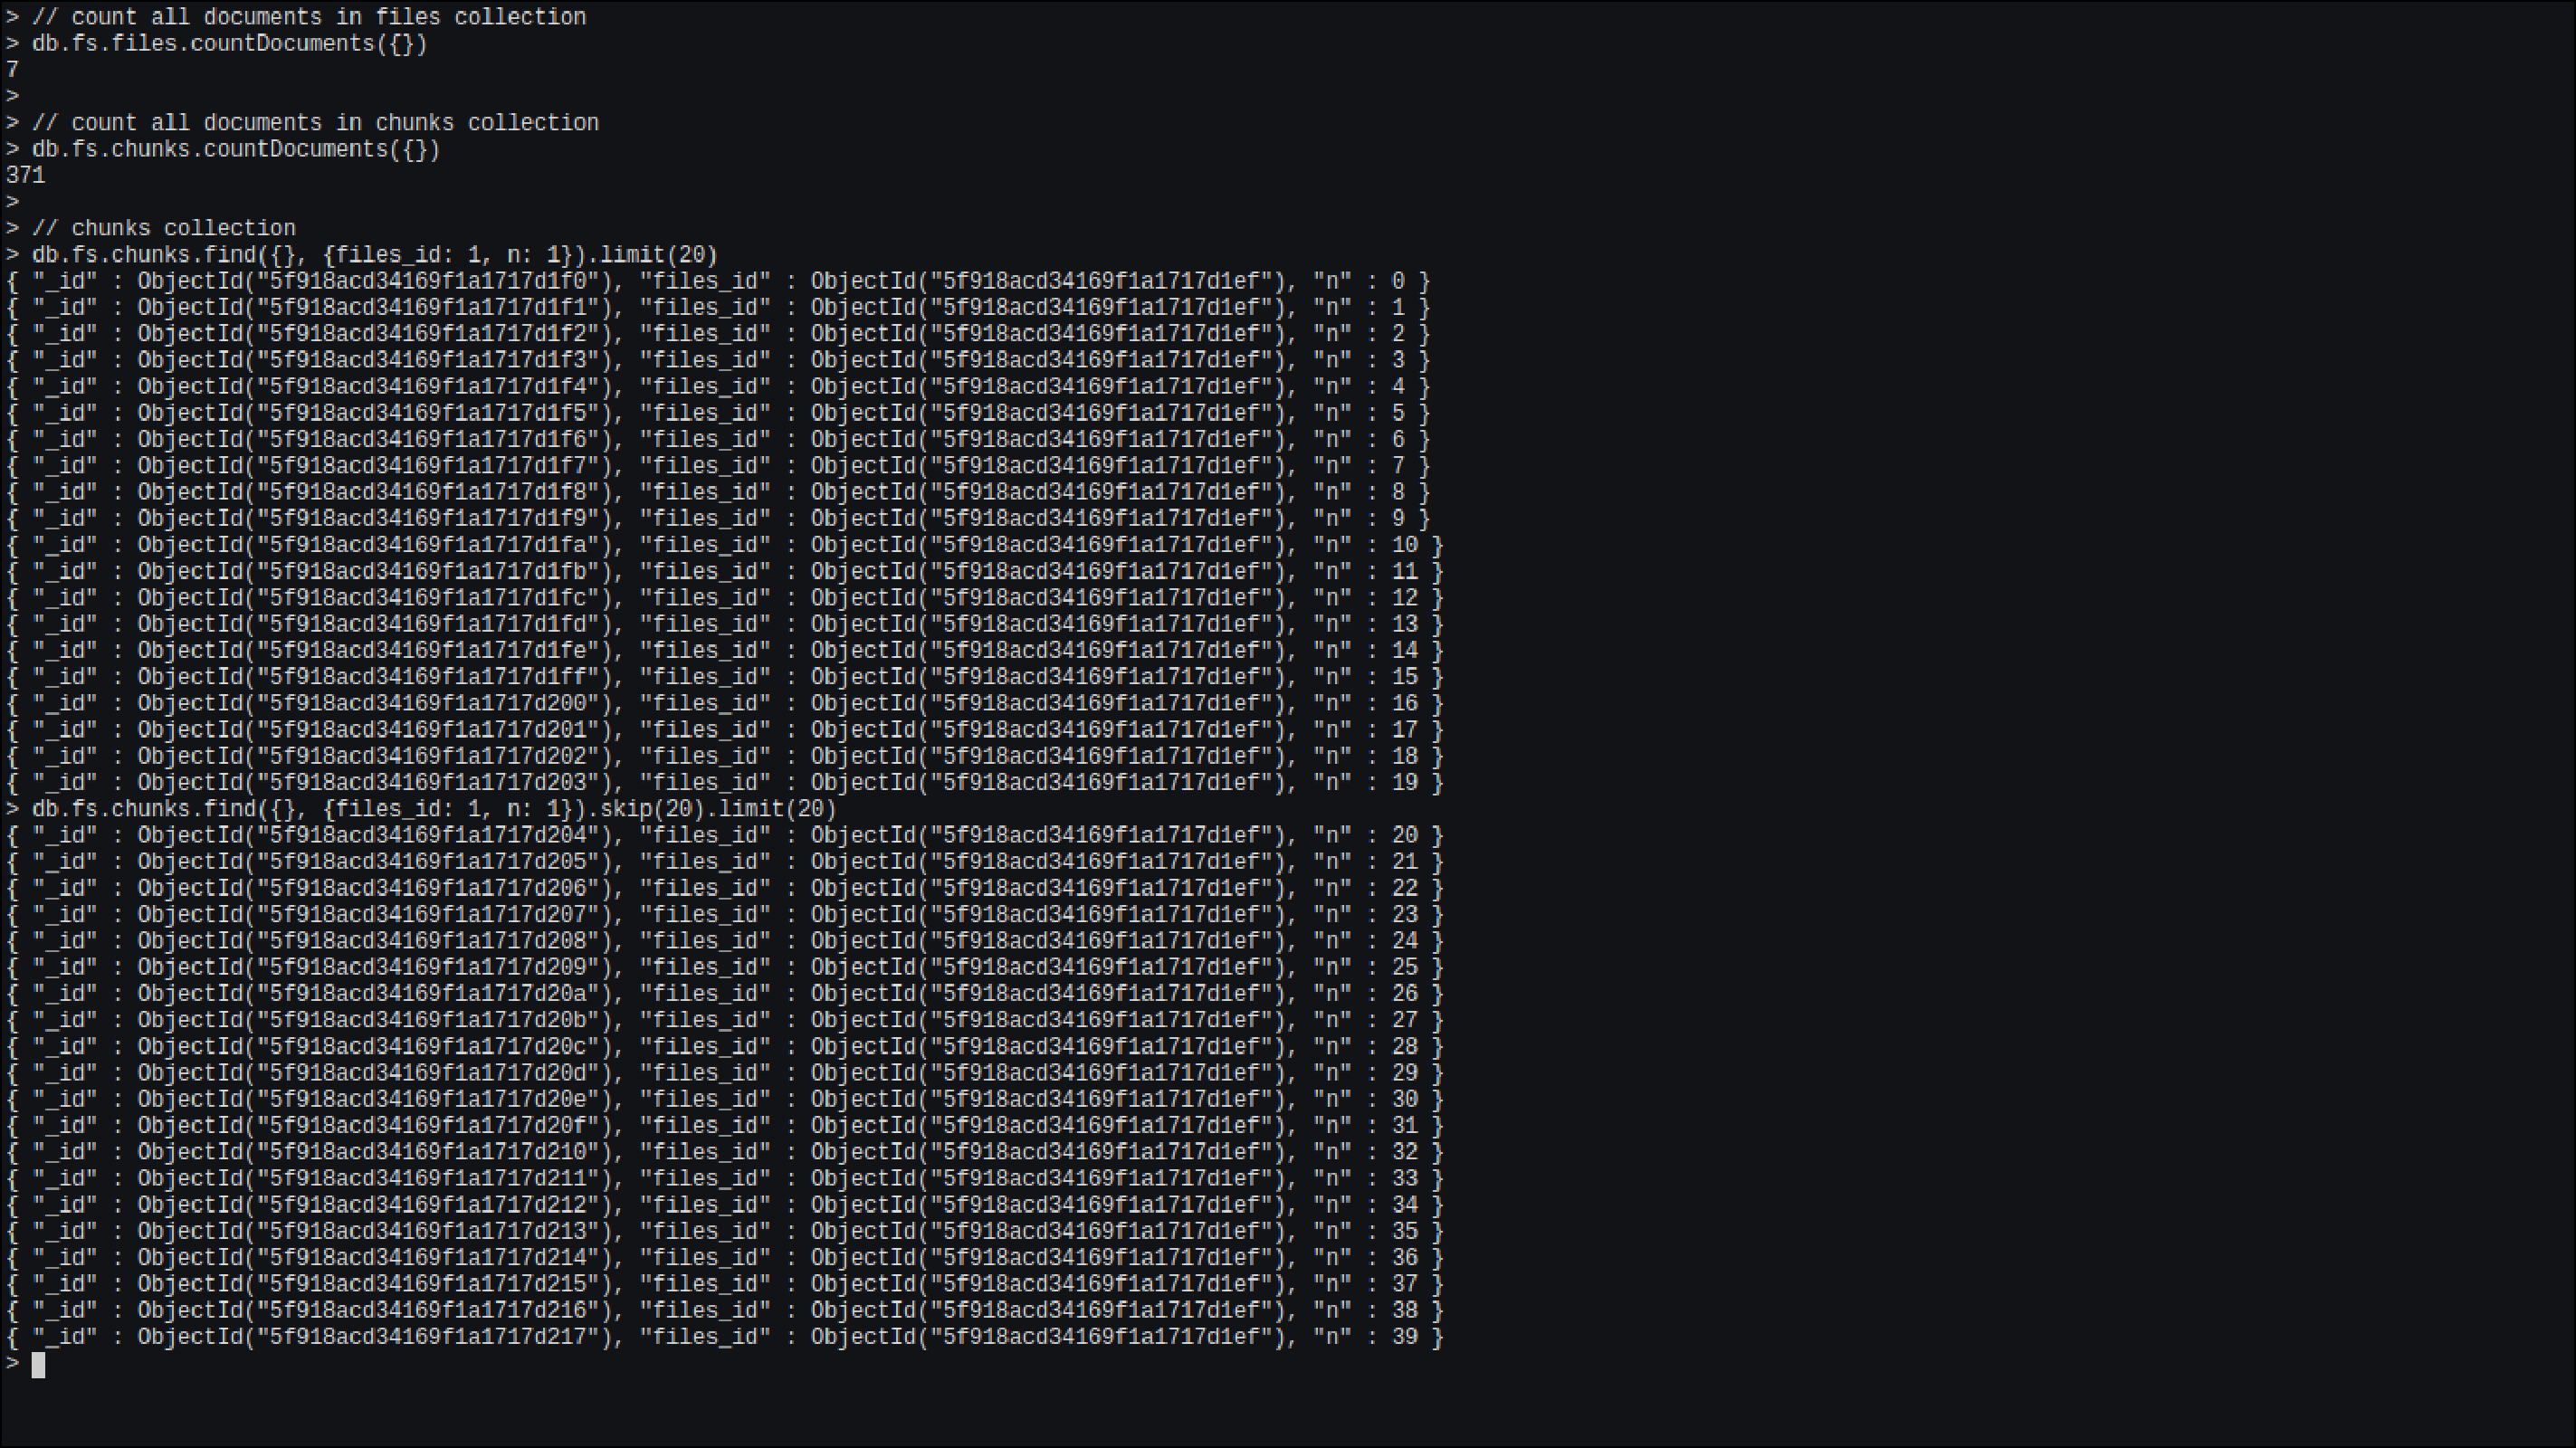
\includegraphics[width=20cm,height=10cm,keepaspectratio]{image4.pdf}
%\centering
%\end{figure}
%
%\pagebreak
%
%{\footnotesize $\$$group}
%%figure_5
%\begin{figure}[ht!]
%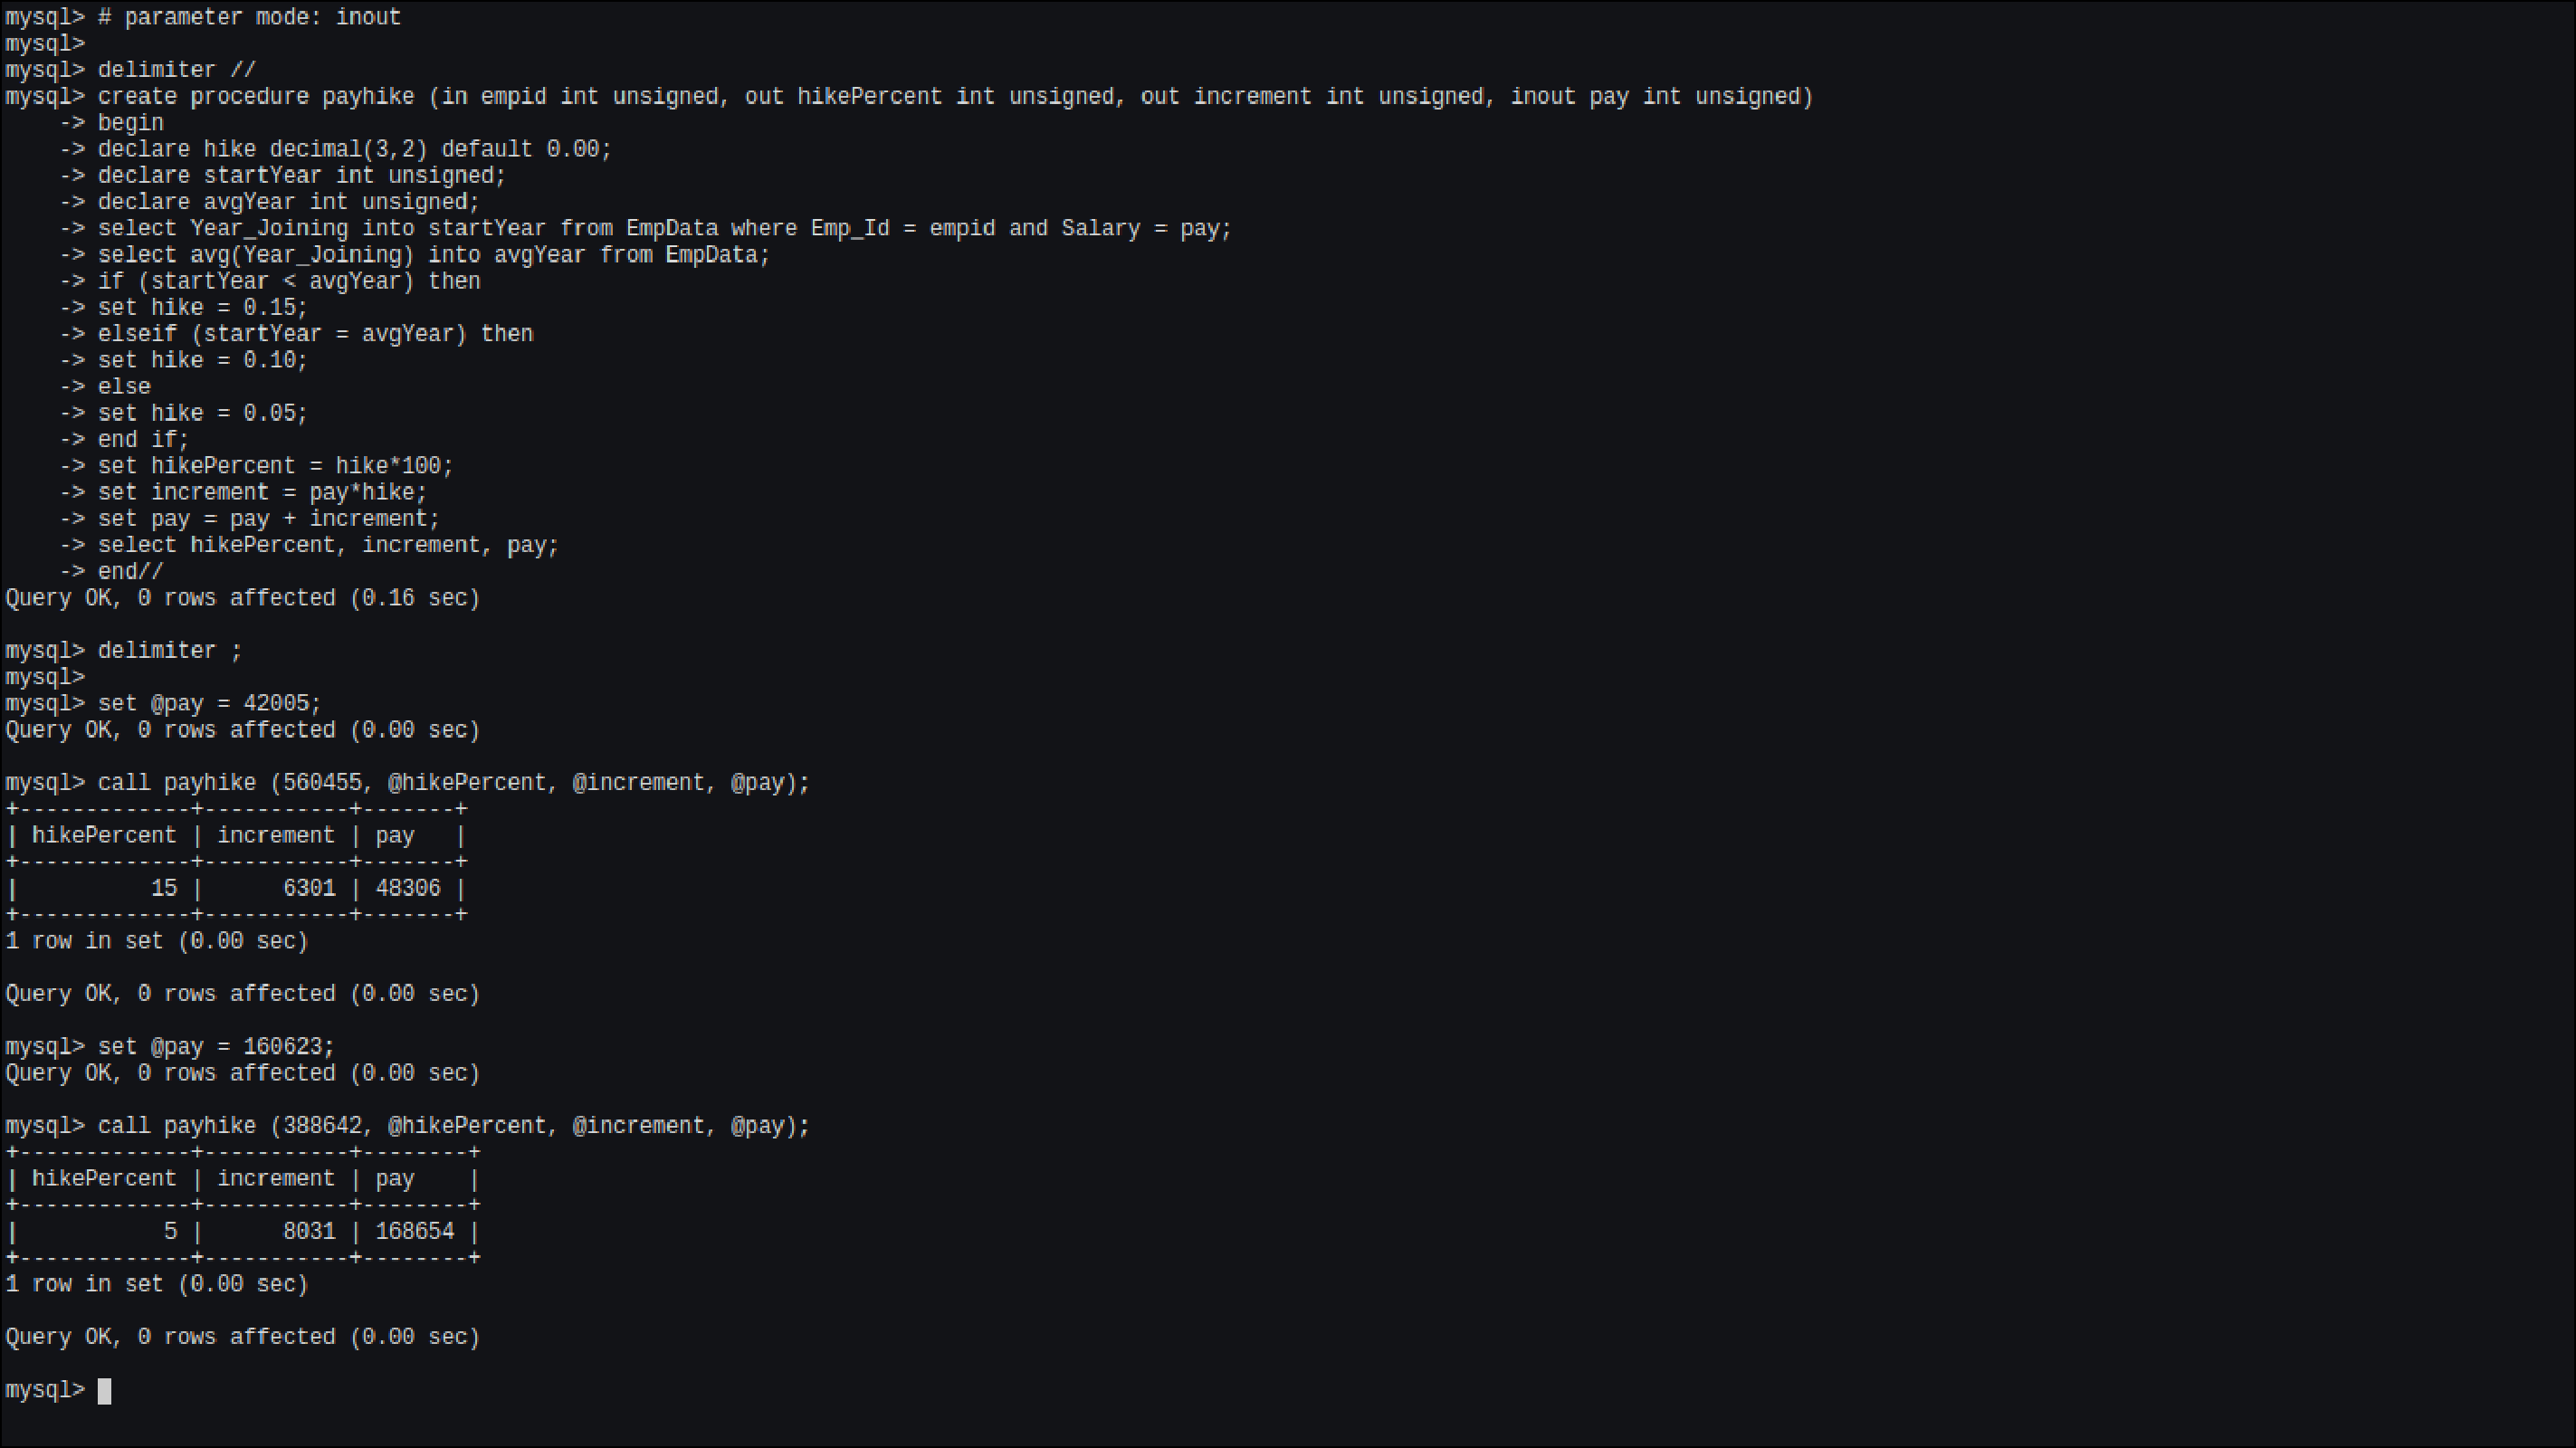
\includegraphics[width=20cm,height=10cm,keepaspectratio]{image5.pdf}
%\centering
%\end{figure}
%
%\vspace{20px}
%
%{\footnotesize $\$$sort}
%%figure_6
%\begin{figure}[ht!]
%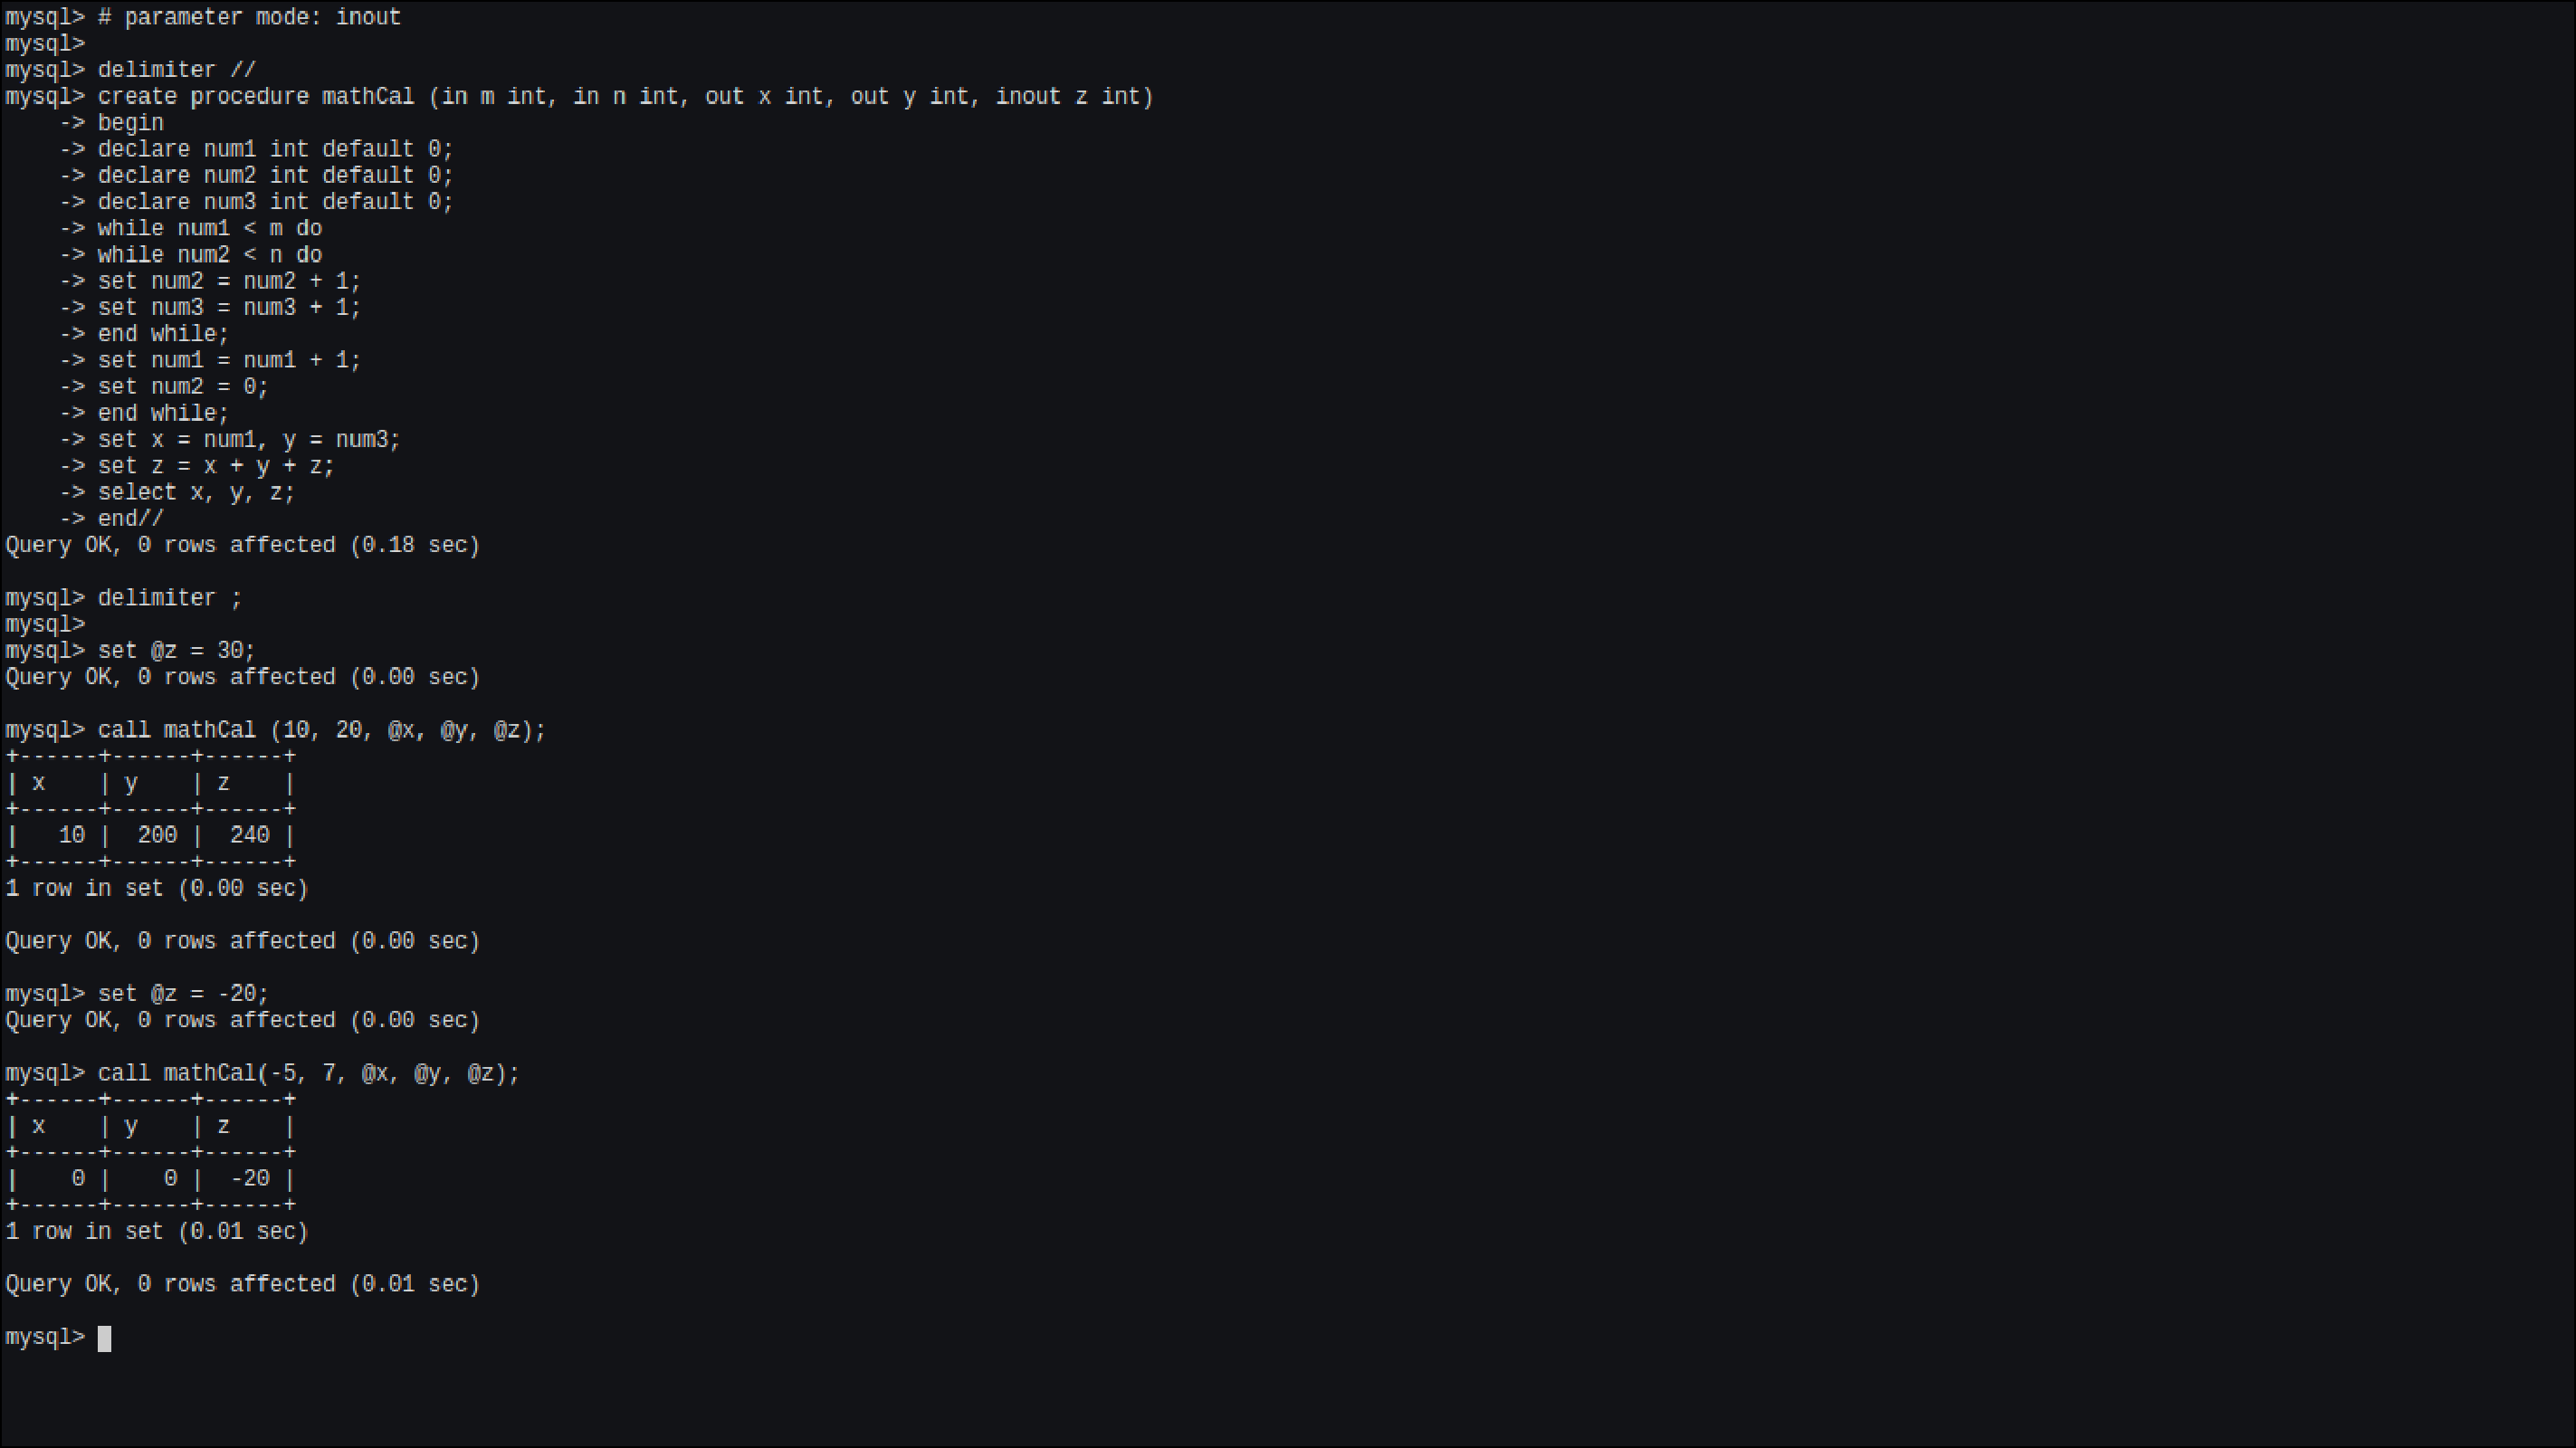
\includegraphics[width=20cm,height=10cm,keepaspectratio]{image6.pdf}
%\centering
%\end{figure}
%
%\pagebreak
%
%{\footnotesize $\$$skip $\&$ $\$$limit}
%%figure_7
%\begin{figure}[ht!]
%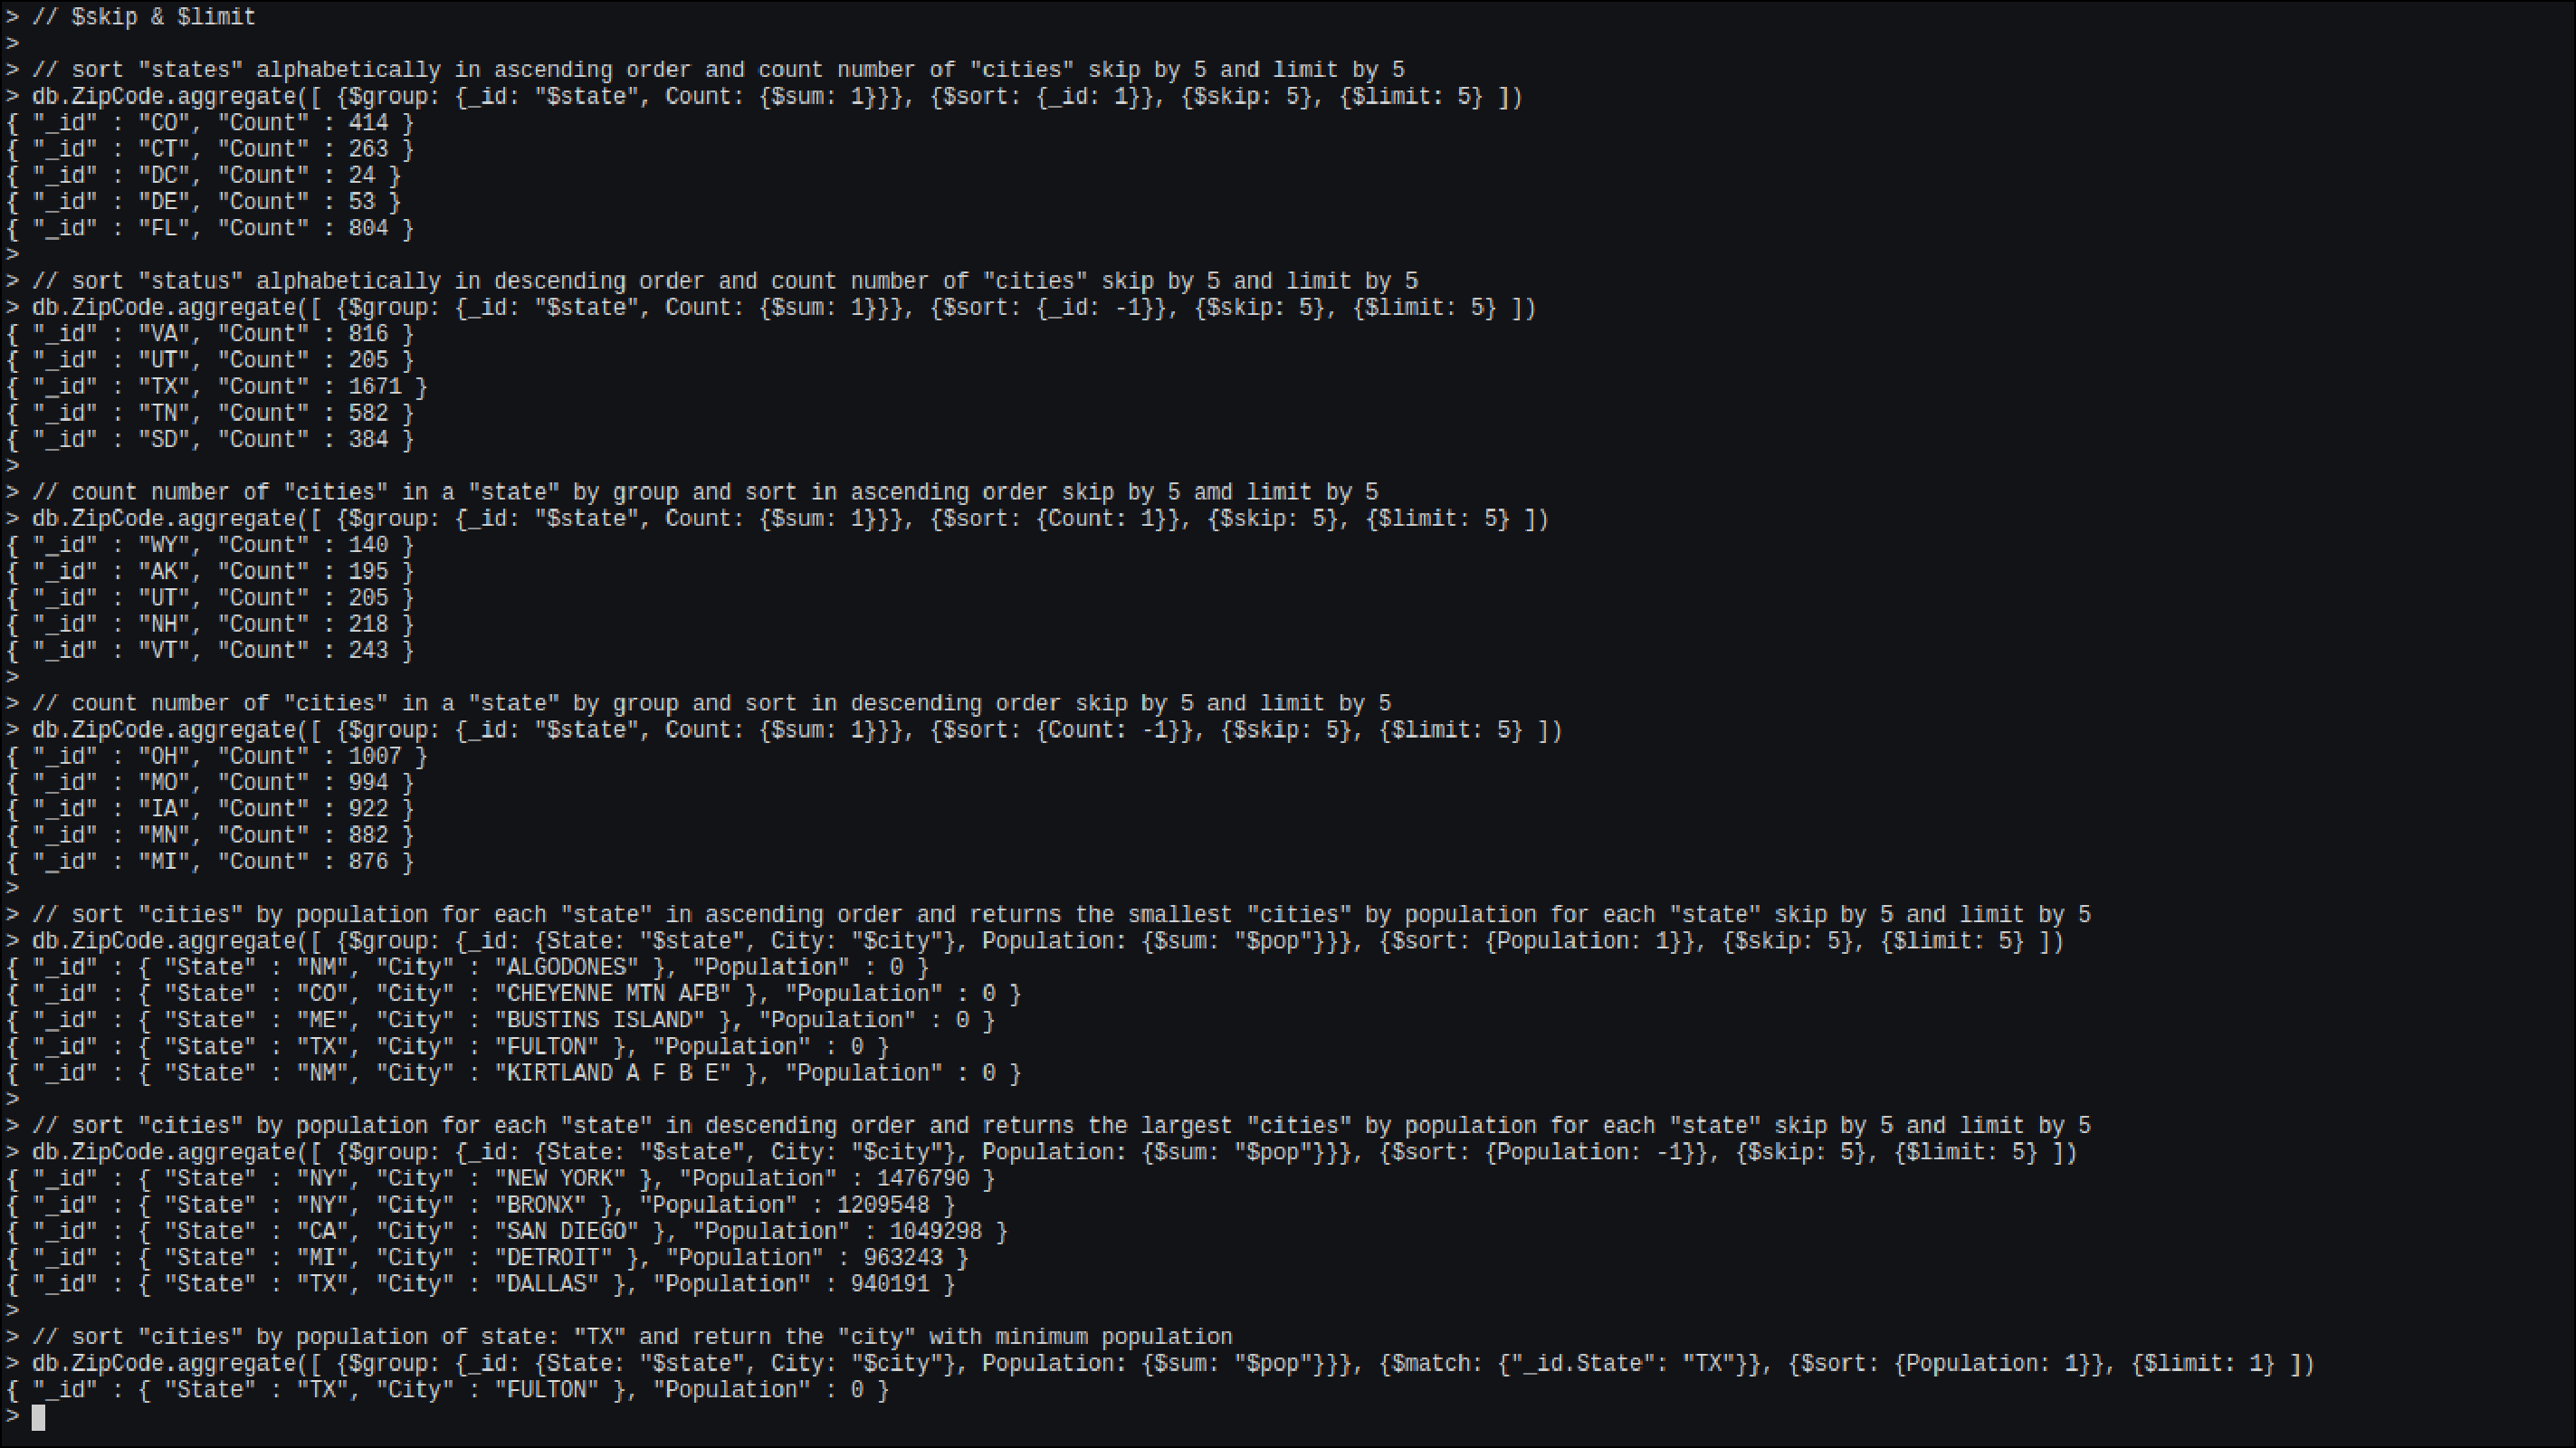
\includegraphics[width=20cm,height=10cm,keepaspectratio]{image7.pdf}
%\centering
%\end{figure}
%
%\vspace{20px}
%
%{\footnotesize $\$$first $\&$ $\$$last and $\$$unwind}
%%figure_8
%\begin{figure}[ht!]
%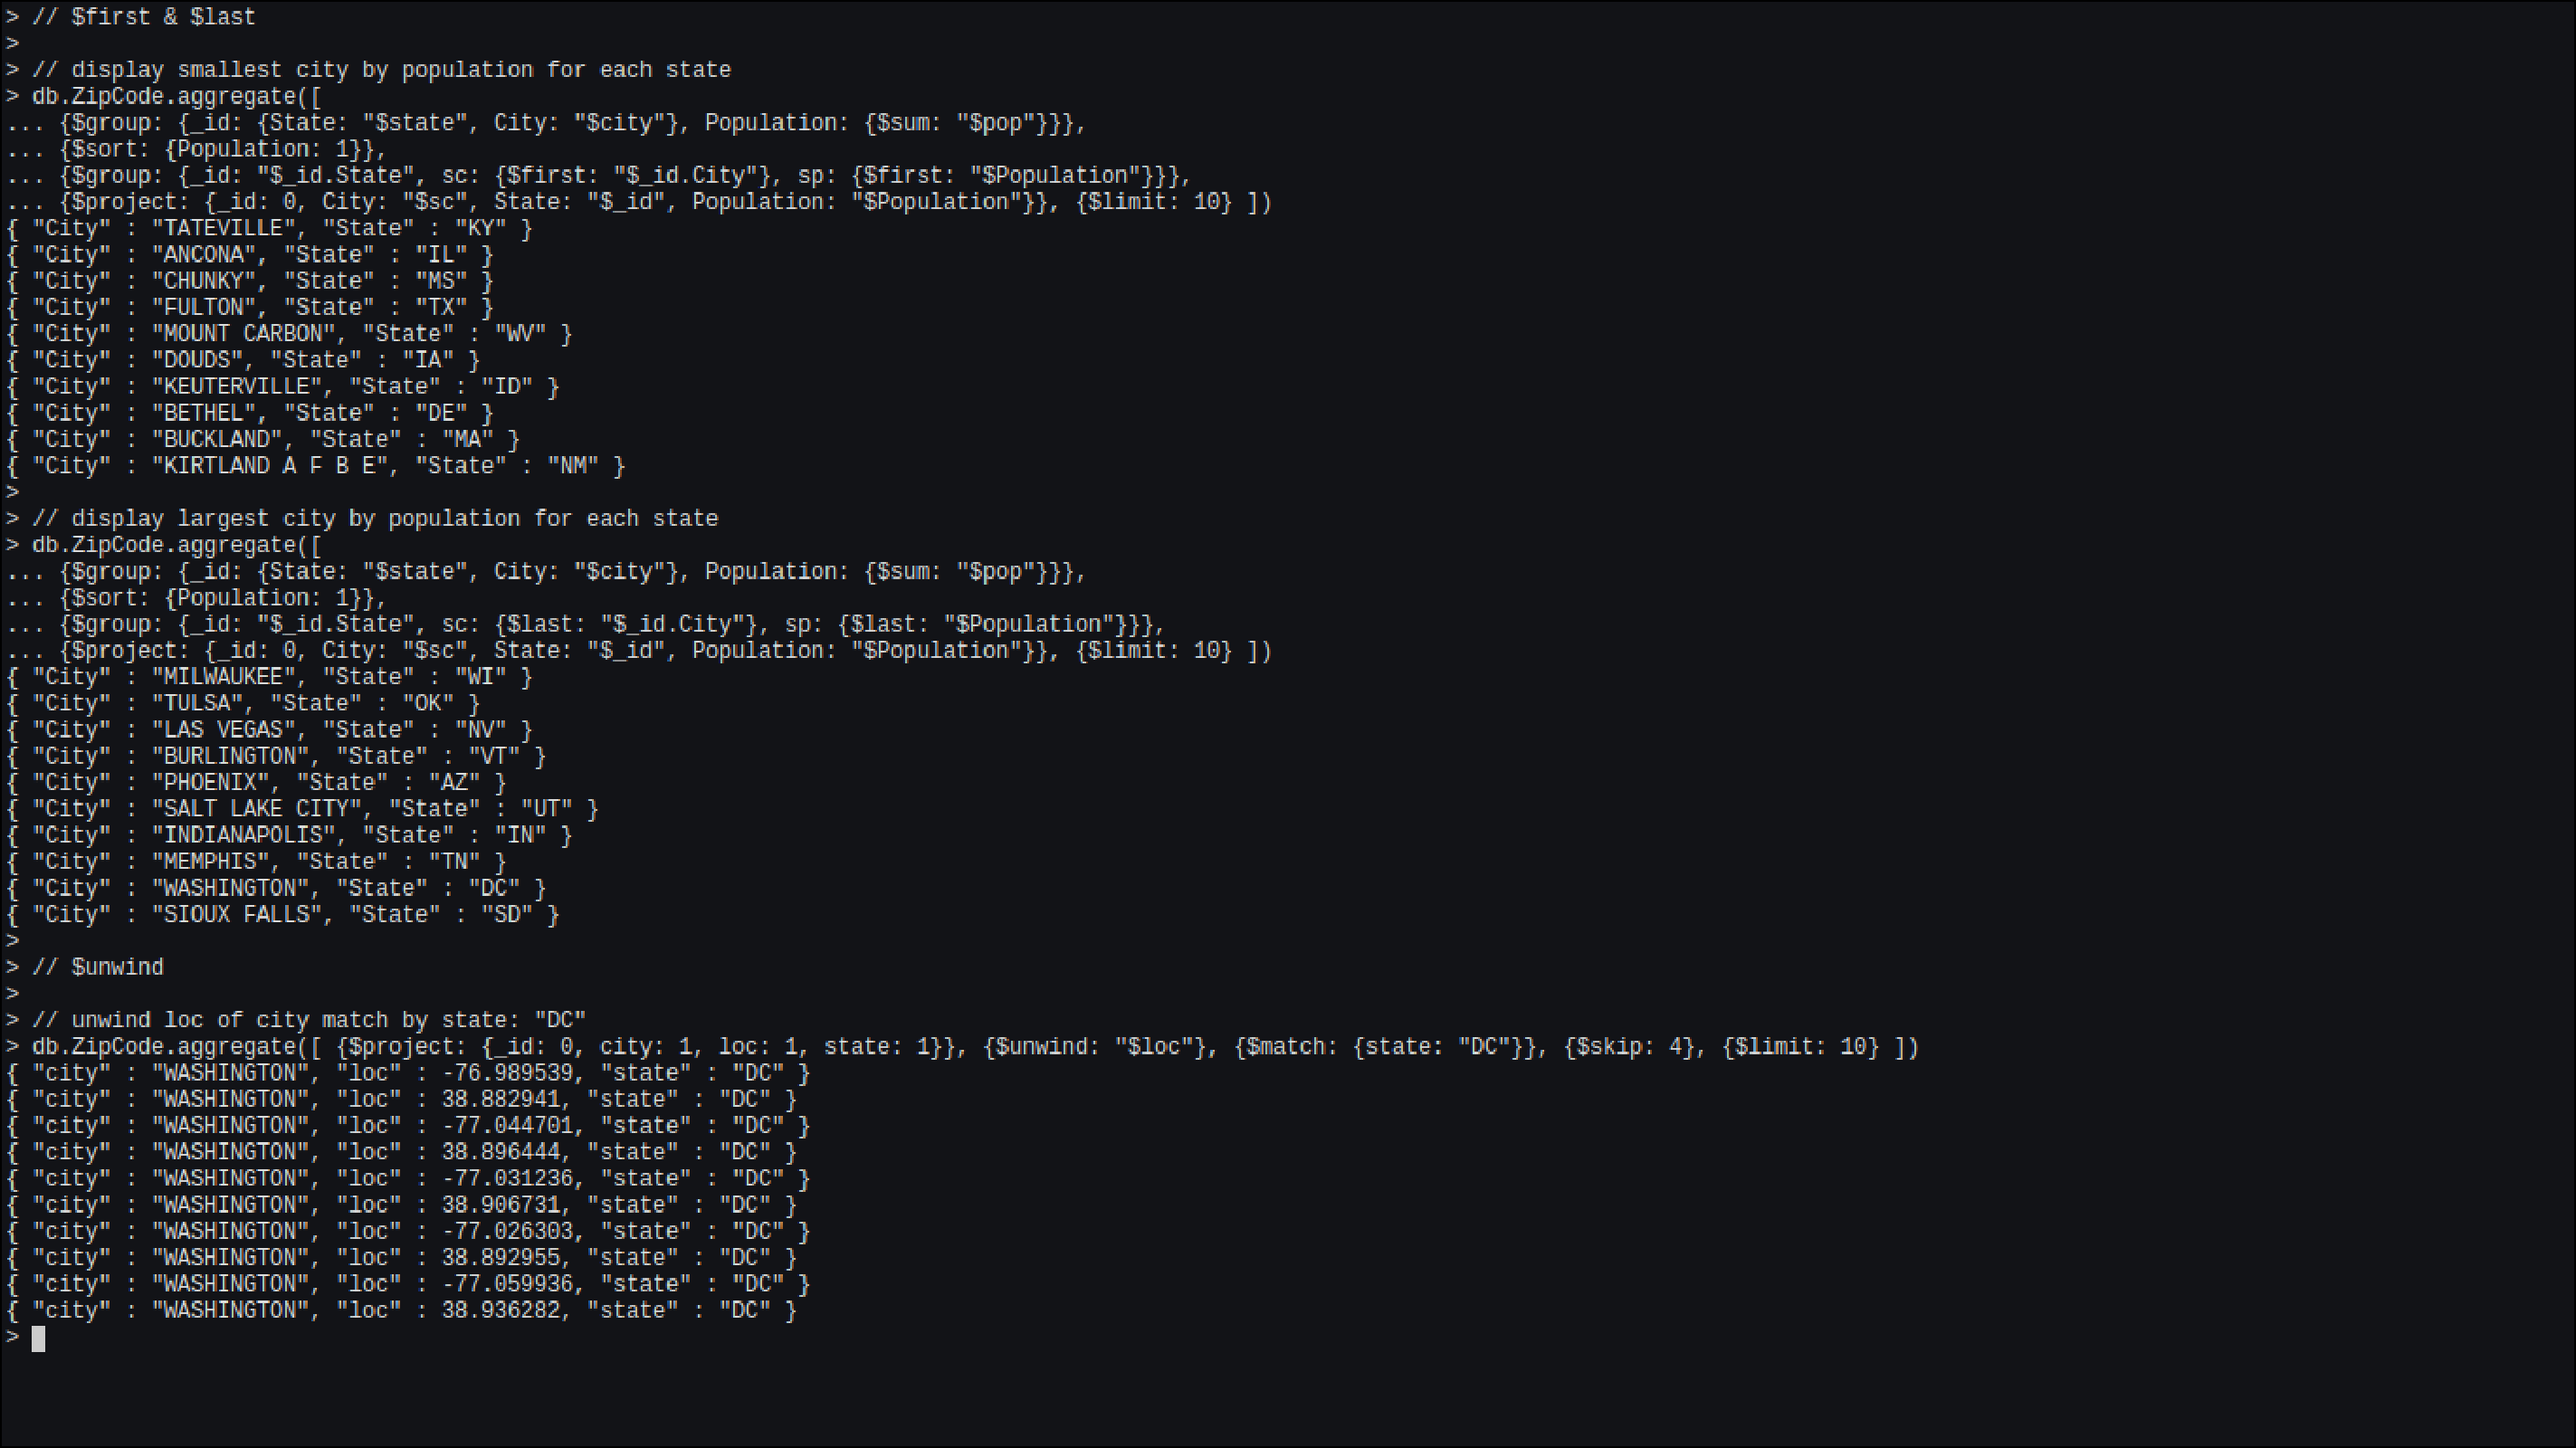
\includegraphics[width=20cm,height=10cm,keepaspectratio]{image8.pdf}
%\centering
%\end{figure}

\end{document}
